\documentclass[11pt,onecolumn]{article}
\usepackage[T1]{fontenc}
\usepackage{times}
\usepackage[hscale=0.8,vscale=0.9]{geometry}
\usepackage[parfill]{parskip}
\usepackage{amsmath}
\usepackage{amsfonts}
\usepackage{graphicx}
\usepackage{xcolor}
\usepackage{subfigure}
\usepackage{wrapfig}
\usepackage{amssymb}
\usepackage{enumitem}


\newcommand{\eat}[1]{}
\newcommand{\todo}[1]{\textcolor{blue}{TODO: #1}}
\setlength{\textheight}{9.05in}
\setlength{\textwidth}{6.5in}
\setlength{\topmargin}{-0.5in}		% -0.5
\setlength{\oddsidemargin}{0in}
\setlength{\evensidemargin}{0in}

%\setlength{\columnsep}{0.2in}   % mike added this

% \setcounter{topnumber}{1}       % another mike: one fig/plot per column
% \setcounter{bottomnumber}{0}    % another mike: and only at the top

% \flushbottom  % Probably not good except for two-side option (facing pages)
% \raggedbottom	% In two-column mode doesn't look so good.

% \parskip .5ex
% \itemsep=-10pt

\makeatletter
%as Latex considers descenders in its calculation of interline spacing,
%to get 12 point spacing for normalsize text, must set it to 10 points
%\def\@normalsize{\@setsize\normalsize{12pt}\xpt\@xpt
%\abovedisplayskip 10pt plus2pt minus5pt\belowdisplayskip \abovedisplayskip
%\abovedisplayshortskip \z@ plus3pt\belowdisplayshortskip 6pt plus3pt
%minus3pt\let\@listi\@listI} 

%need an 11 pt font size for subsection and abstract headings
\def\subsize{\@setsize\subsize{12pt}\xipt\@xipt}

%make section titles bold and 12 point, <2 blank lines before, <1 after
\def\section{\@startsection {section}{1}{\z@}{18pt plus 2pt minus 2pt}
{6pt plus 2pt minus 2pt}{\large\bf}}

%make subsection titles bold and 11 point, 1 blank line before, 1 after
\def\subsection{\@startsection {subsection}{2}{\z@}{12pt plus 2pt minus 2pt}
{3pt plus 2pt minus 2pt}{\subsize\bf}}

\def\subsubsection{\@startsection {subsubsection}{3}{\z@}{11pt plus 2pt minus 2pt}
{3pt plus 2pt minus 2pt}{\normalsize\bf}}

% \def\subsubsection{\@startsection {subsubsection}{3}{\z@}  
%  {11pt plus 2pt minus 2pt}
%%  {3.25ex plus 1ex minus .2ex}
%  {-1em}
%  {\reset@font\normalsize\bf}
%}

\makeatother

\setlength{\parindent}{0pt}
\setlength{\parskip}{0.25em}
%\setlength{\parindent}{0.5pt}
%\setlength{\parskip}{0.25em}
\begin{document}
\include{weld-defns}
\title{CRII:III: Composing Process Knowledge using Semantic Roles}
\author{Niranjan Balasubramanian}
\maketitle
\newpage
\thispagestyle{empty}
%%!TEX root = summary-only.tex
\begin{center} 
	{\bf CRII:III: Composing Process Knowledge using Semantic Roles}\\
	{Niranjan Balasubramanian, Stony Brook University}

 \end{center}

Large-scale text resources and fact databases have spurred significant advances 
in AI systems that answer factual questions  (e.g., "When was Bill Clinton born?").
To address more challenging problems that go beyond factual answer retrieval,
AI systems need to be able to reason about general scenarios. 
They need to know general truths or generalities and how to apply them to specific situations. 
Acquiring this type of general knowledge and using it to reason effectively remains a huge challenge.

We explore this challenge for reasoning about {\em processes} in order to answer
questions about specific scenarios involving them. 
In particular we propose to compose knowledge about processes in terms of semantic roles (e.g., What is undergoing the process? What is the result? etc.). We develop solutions to automatically construct a large repository of simple process knowledge, and demonstrate its use to answer process questions that go beyond fact lookup. 

Existing lexical semantic resources provide similar forms of semantic knowledge about general open-domain actions but lack coverage on scientific processes. FrameNet, for instance, does not have entries for nearly half of the processes described in 4th grade science exams. The coverage is likely worse for higher grade levels with deeper knowledge domains. 

%. For example, PropBank and FrameNet provide role knowledge about open-domain actions and have been successfully used in information extraction and open-domain QA. While they provide exhaustive coverage for open-domain actions (verbs), their coverage on processes in the science domain is lacking. FrameNet, for instance, does not have entries for nearly half of the processes described in 4th grade science exams. The coverage is likely worse for higher grade levels with deeper knowledge domains. 
In response we propose to investigate methods to automatically construct a large repository of simple semantic role based knowledge about processes. Adapting existing semantic role labeling systems to work well on new domains is difficult. We take a different approach. Our key premise is that rather than building a semantic role labeler that works well on any sentence, we proactively gather sentences that convey information in expected constructs. We propose a framework that combines techniques from extraction and joint inference for finding semantic roles and iteratively expands its knowledge to discover roles on its own.
Specifically, we will make three main contributions:
\begin{itemize}[noitemsep,nolistsep]
\item The first comprehensive, large-scale {\bf knowledge base of processes} in the grade science domain, describing the roles
      and changes involved in that process.
\item Methods for {\bf automatic extraction of process knowledge} using information extraction and joint inference.
\item A framework for {\bf iterative knowledge expansion}, which allows the system to discover new roles
     involved in a process and expand the process representation to accommodate them.
\end{itemize}

{\bf Intellectual Merit} 

This work investigates a new direction in acquiring semantic roles by targeting sentences that express information in expected ways. The work will lead to better understanding and advancement of cross-sentence alignment of semantic roles and collective labeling. This work will push understanding on continuous learning (similar to the NELL project for relation extraction) with the iterative expansion methods and increase understanding of the connection between regularities of syntactic realizations and semantic roles. Overall the project also contributes to advances in leveraging unlabeled data and methods for balancing representational needs against extraction capabilities.

{\bf Broader Impact}

Automatic knowledge extraction is fundamental to advancing Artificial Intelligence. 
This work contributes towards building systems capable of understanding knowledge in texts and reason with them.
Better reasoning systems help information access and reduce information overload thereby accelerating research and discovery, 
as well as serve the information needs of the population at large.

{\bf Keywords} Knowledge extraction, Semantic Role Labeling, Information Extraction, Question Answering


% -- In order to scale, we will investigate methods for automatically determining which roles are applicable for a particular process. Prior works have either relied on fully supervised training data to specify roles~\cite{} or have relied on clustering of syntactic functions to automatically induce roles~\cite{}. We propose an intermediary solution that aims to determine which set of roles (from a pre-specified role vocabulary) applies to the process. The intuition is that there are some general purpose notions such as {\em direction}, {\em medium}, {\em change} etc that are common to many processes.
%	
\eat{Knowledge-intensive benchmarks including standardized grade-level science exams~\cite{clark2015elementary}, 
textual entailment~\cite{dagan2010recognizing}, and reading comprehension tasks~\cite{richardson2013mctest} have renewed interests in automatic knowledge extraction and reasoning. 
These tasks motivate reasoning-based systems that go beyond simple retrieval and syntactic structure matching~\cite{clark2014:akbc,chb2013:akbc, khot2015:emlnlp}. 

Effective semantic representations of relevant information is critical for making significant advances in building such systems. 
Semantic role-based representations have shown promise for open-domain factoid question answering~\cite{shen2007using, pizzato2008indexing}. 
Some of the knowledge required for grade-level science exams are naturally expressed via semantic roles.
Consider the following example from an actual 4th grade science exam.

{\em When plants use stored sugar for energy, they go through a process called \\
(A) photosynthesis (B) transpiration (C) respiration (D) perspiration.}\\

{\em Photosynthesis} and {\em respiration} both involve sugar and energy. 
Photosynthesis converts light energy to sugar, whereas (cellular) respiration releases energy in the sugar by breaking it down. 
Not surprisingly these processes are described using similar words, which makes bag-of-words style reasoning unreliable. 
Understanding the different roles that energy and sugar play in these processes is key to effective reasoning.
Such semantic roles are critical for performing chained automated reasoning. 

Several existing resources provide semantic representations of general open-domain actions e.g., FrameNet, PropBank, and VerbNet. 
However, these resources do not adequately cover many of the scientific processes. 
FrameNet, for instance, does not have entries for nearly half of the processes described in 4th grade science exams. 
The coverage is likely to be worse for higher grade levels.

We propose to build a knowledge base about physical, chemical, and biological processes from their textual descriptions. 
The central idea is to automatically compose a semantic representation using a pre-determined vocabulary of semantic roles. 
Having identified the roles of interest, we will seek out sentences that express these roles and build extractors for these roles via bootstrapping.
%\footnote{We call these extractors rather than semantic parsers, since the goal here is to build knowledge about these processes and  not necessarily to build a parser that can reliably identify {\em all} semantic roles expressed in a sentence.} 
We will conduct intrinsic and external evaluations. 
We will create a manual target representation for intrinsic evaluation, and use the 4th grade science questions as an external application.

}     % A. Project Summary - 1 page
\newpage
\tableofcontents    % B. Form 1359
\thispagestyle{empty}
\setcounter{section}{0}
\setcounter{page}{0}
\newpage
%
\setcounter{page}{1}
% !TEX root =  main.tex
\section{Introduction}

AI systems have achieved impressive success with answering factual questions 
(e.g., "When was Bill Clinton born?"), using information from large-scale text or database resources~\cite{berant2013semantic,fader2014open,bordes2014open,reddy2014large,watson}. 
To scale more challenging problems that go beyond factual answer retrieval~\cite{richardson2013mctest,clark2015elementary,berantSrikumar14}, 
AI systems will need the ability to reason about the world. In particular they need knowledge of generalities 
and how it applies to the specific situations. Despite significant advances in AI, acquiring 
general knowledge and using it to reason effectively remains a huge challenge.
%and applying general knowledge about the world remains a huge challenge. 

We propose to investigate this challenge in the context of learning and reasoning about {\em processes}.
Knowledge about processes is a fundamental to part of our understanding of the world and it is 
essential to make predictions and answer questions about specific scenarios involving them.
Our goal is to develop solutions to automatically construct a large repository of simple process knowledge 
automatically, and demonstrate its use to answer process questions that go beyond fact lookup. 

\subsection{Motivation}
We motivate the need for process knowledge using an example from an actual 4$^{th}$ grade science exam.
\begin{figure}[hbt]
	\begin{center}
	\vspace{-1em}
	% 12.08 x 1.90
	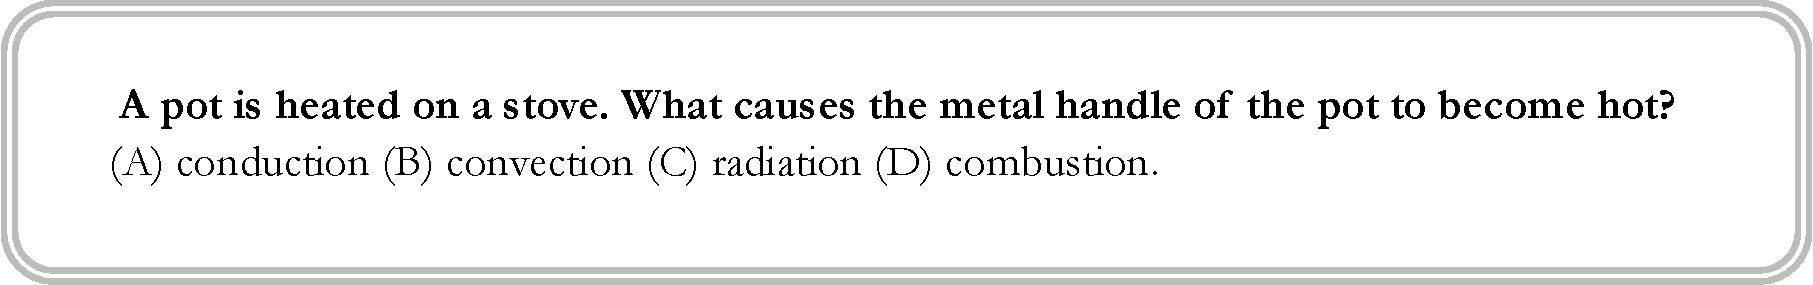
\includegraphics[width=6.04in,height=0.95in]{figures/single-question-stretch.pdf} 	
	\vspace{-1em}
	\end{center}
\end{figure}

The question tests the ability to recognize a specific scenario involving a heat transfer process.
To establish that conduction is the cause, a reasoning system must establish that there is some heat transfer happening through {\em direct contact}. 
We envision a system that first interprets the scenario and apply its knowledge about the heating process and the conduction process. 
In this case, the system needs to first identify {\em what is being heated} (the pot), and {\em what is the purported result} of the heating (the pot handle becoming hot). 
Then, knowledge about {\em heating} should allow it to conclude that the thing being heated (the pot) will become hot. 
Knowledge about {\em conduction} should suggest that anything {\em in direct contact} with a hot object (the pot handle) should also become hot.
Combining these bits the system can verify that the described scenario indeed matches the conduction process.
Replicating this type of reasoning requires knowledge about conduction and heating in a suitable computational representation.
\todo{[Reads very rough.]}
%Specifically the knowledge about conduction should convey that there are two entities that are in direct contact, one of which is being heated or is hot, 
%and the result of conduction is that the other object also becomes {\em hot}. 

At a high level the main bits of required knowledge are: what is undergoing the process, what is the result, what is the main action etc.
These bits of information are naturally encoded as semantic roles.
PropBank~\cite{kingsbury2003propbank} and FrameNet~\cite{baker1998berkeley} are two of the highly successful efforts which provide this kind of semantic role based knowledge.
They have spurred tremendous advances in automatic semantic role labeling and their applications~\cite{gildea2002automatic,surdeanu2008conll,feizabadi2015combining,roth2015context}.
While these resources provide exhaustive coverage for modeling general open-domain actions, they only provide partial coverage on processes in the science domain.
FrameNet, for instance, does not have entries for nearly half of the processes described in 4th grade science exams. 
The coverage is likely worse for higher grade levels with deeper knowledge domains. 

In response we propose to investigate methods to automatically construct a large repository of simple knowledge about processes. Specifically, we will make three main contributions:
\begin{itemize}
\item A method for {\bf automatic extraction of process knowledge} that combines extraction and joint inference.
\item A framework for {\bf iterative knowledge expansion}, which allows the system to discover new roles
     involved in a process and expand the process representation to accommodate them.
\item The first comprehensive, large-scale {\bf knowledge base of processes}, describing the roles
      and changes involved in that process.
\end{itemize}

To provide a concrete test-bed for development and evaluation purposes, we will initially
develop this in the domain of elementary science, and evaluate it using unedited science
exam questions about processes. We expect the resource to be useful to other researchers
working in the areas of natural language processing, text processing, and question answering.

\section{Proposal Synopsis}

%\subsection{Representation}

Our primary motivation is to design a representation that effectively supports reasoning while also being amenable for automatic extraction.
We target a simple\footnote{Process knowledge is typically complex with sub-events, and temporal dependencies. They are beyond the scope of this investigation.} form of  knowledge that captures information about the entities involved and their semantic roles within the process.

We turn to the inferential needs of the target application to guide our choices.
Our preliminary work in this domain suggests a mix of {\bf pre-specified semantic roles} that apply to many processes, 
and a set of {\bf automatically induced roles} that are process specific~\cite{louvan2015:kcap}. 
We also find that we need both {\bf definitional} -- describing the key classes of entities and types of actions involved -- and {\bf instance level} knowledge about specific scenarios in which the processes occur -- providing details on the specific entities and actions. 

%process knowledge required is quite diverse, some of which is definitional in nature -- describing the key classes of entities and types of actions of a process. Others are specific to certain occurrence of the processes in specific situations or contexts -- providing details on the specific entities and actions. 
%By leveraging a common vocabulary we expect to gain from shared learning for the same roles across different processes.
%We propose to compose knowledge about each process using a set of pre-determined vocabulary of semantic roles and derive additional new roles automatically as needed.
%While many competing role sets exist, we propose a role vocabulary that covers most inferential needs in the target application~\cite{louvan2015:kcap}.

\begin{figure}[hb]
	\begin{center}
	%13.5 x 15.15
	%20.01 x 6.78
	%18.79 x 6.78
	%13.36 x 6.78
	\includegraphics[width=4.453in,height=2.26in]{figures/processkb-snippet-noqp.pdf} 	
	\caption{\label{fig:kbsnippet} 
	{An example entry for the process {\em thermal conduction}.}
	}
	\end{center}
\end{figure}

Figure~\ref{fig:kbsnippet} shows an example for the envisioned knowledge. 
The table includes a set of pre-specified general purpose roles such as {\em Undergoer}, {\em Enabler} and also a process specific role {\em Medium} that is automatically derived from inspecting sentences that describe the process. In addition to the {\em instance} role fillers, it also includes {\em definitional} type information which encodes class level information where possible.

\subsection*{Research Questions}
%Similar to FrameNet we propose to determine roles with respect to the semantics of the process rather than with respect to the specific verb (or predicate) that is used to describe the process.
%This canonicalization is desirable as it reduces reasoning time burden by eliminating need for steps that only establish equivalence of information realized via different predicates.
% %The need for a canonicalized representation precludes the direct use of existing annotations or tools built for PropBank.

There are many research challenges in automatically extracting this knowledge from text.
\begin{itemize}
\item SRL systems typically rely on large amounts of training data in order to generalize over sparse features. How can we leverage the abundance of information on the web to reduce the need for large training data?
\item A priori it is not clear how to identify which set of sentences are likely to contain relevant information.  How to gather sentences that convey the necessary knowledge? 
\item How do we account for process specific roles? 
\end{itemize}

Our investigation aims to answer these questions. 

\subsection{Automatic Extraction of Process Knowledge}
General semantic role labeling task is challenging because of the lexical and syntactic variations in role realizations. 
Handling the variations requires learning from large amounts of training data, which is laborious and requires expert labor.
%Also as discussed earlier, existing semantic resources such as FrameNet or PropBank cannot be directly used for training as they do not cover the target concepts.

Our key premise is that to gather role knowledge we don't need a semantic role labeler that works well on all sentences. 
We are interested in role acquisition and not role interpretation.
We exploit the abundance and variety of information available on the web to target extraction from 
sentences that convey the same information in expected (easy to extract) constructs and 
use joint inference to further improve performance. Our approach includes:
\begin{itemize}
\item {\bf Targeted Pattern-based Extraction} --  We build a simple pattern-based local role extractor augmented with a classifier.
Using a set of manually constructed query patterns we search the web to find sentences and extract role fillers.
A simple classifier then assesses if the extraction is valid.
%Beginning with a set of manually constructed query patterns we search the web to find sentences that match these patterns.
%For instance "<process name> causes <x>" is a simple pattern that can be used to find the {\em result} role for a process. 
Unlike traditional SRL tasks, here we have a strong expectation of the type of role and where the filler is likely to be located.
This expectation allows us to design simple structural features that generalize better across different roles and processes, 
thereby reducing need for large amounts of training data.

\item {\bf Joint Inference Across Sentences} -- We propose a joint inference model that operates over multiple sentences to avoid errors in the local extraction.
Despite the targeted acquisition, local sentence-level extraction alone is not adequate, because not all patterns are unambiguous. 
For example, "evaporates into <x>" extracts steam, a {\em result}, as well as atmosphere, a {\em location}. 
Redundancy and variety of expression on the web can help us: If the {\em atmosphere} were in fact a {\em result} then we might expect to see other sentences
where it is expressed as a result with unambiguous patterns. We propose a joint inference formulation that favors roles 
minimizing disagreements in labels for similar text spans in similar sentences.

%Because our goal is to acquire knowledge about a process, we turn the variety of expression on the web to our advantage. 
%If the {\em atmosphere} were in fact a {\em result} then we might expect to see other sentences
%where it is expressed as a result with unambiguous patterns.
%Prior work proposed Integer Linear Program (ILP) based approach for joint inference for roles {\em within} sentences.
%We build upon this work to find an assignment of roles that maximizes the sum of extraction confidences, 
%while also minimizing disagreements in labels for similar text spans in similar sentences.
\end{itemize}

\subsection{Iterative Knowledge Expansion} 
Determining the best set of knowledge bearing sentences {\em a priori} is extremely difficult. 
The quality and scope of the extracted knowledge is effectively determined by the set of sentences retrieved by the query patterns.
The query patterns may have limited coverage in some cases especially for roles that were not part of the pre-specified vocabulary.
We propose an iterative expansion of the knowledge to improve coverage of existing roles, and to discover new roles. 
An inspection of the gathered knowledge can provide valuable guidance in expanding and refining the knowledge.
We propose to investigate methods to 1) assess the coverage of the roles, 2) induce new roles by identifying consistently repeated arguments that don't fit existing roles,  
3) bootstrap extractors and query patterns using relevance feedback techniques, 4) refine the knowledge by organizing the knowledge in clusters of scenarios/instances.

\subsection{Knowledge Base of Processes}

Our target domain is grade level science. 
Based on initial analysis we estimate to generate about entries for around 2000 processes encompassing simple physical, chemical, biological, and other natural processes in this domain. 
As part of the proposed work, we propose to curate a subset of this knowledge base. Recent work has shown an effective question-based mechanism for acquiring semantic role labels
via crowd sourcing~\cite{hequestion}. To foster further research, we will release the knowledge base, and open source the code, and host web services that will allow dynamic construction of knowledge for new unseen processes. We anticipate this knowledge base will also be useful for QA in the science domain, for communities interested in AI systems, 
and to the semantic role labeling community at large.

The proposed methods will be evaluated for intrinsic quality and external utility. For internal evaluations we will perform manual evaluation of the resulting KB. 
As an external evaluation we will use the knowledge base for answering process recognition questions.

The remainder of this proposal provides details on these three main contributions.
%As part of the evaluation, {\bf we will also create a large scale curated KB, which relies on correcting the outputs from the system, rather than careful annotation of each sentence}. 
%We will also generate a gold standard of the desired roles and role fillers for evaluating coverage. As an external evaluation we will use the knowledge base for answering process recognition questions. All the %resources and evaluation test beds will be shared with the research community for further research.


\eat{\subsection{Prior Work and Contributions}

The motivation and direction for this proposal stems directly from our prior work on grade science exams.  Our earlier work studied knowledge requirements~\cite{chb2013:akbc}, developed inference-supporting rule knowledge bases~\cite{clark2014:akbc}, and investigated sophisticated state-of-the-art probabilistic reasoning methods for QA~\cite{khot2015:emlnlp}. Our ongoing preliminary work investigated the value of a handful of semantic roles in answering process recognition questions and identified the knowledge, representation, and reasoning gaps~\cite{louvan2015:kcap}. This proposal aims to address the central challenges that we've identified through these prior works.

Upon successful completion this project would have made the following contributions:
\begin{itemize}
\item {\bf Semantic Resource for Grade-level Science} -- The knowledge base we build will cover process in grade-level science and will be made available to the public and the academic community 
for fostering research in automatic reasoning systems. To foster further easy exploration, all the code will be open sourced and we will also host a web service that will dynamically compose the knowledge for new unseen processes. 
\item {\bf Targeted Acquisition and Local Extraction} -- A targeted acquisition method that gathers sentences expressing roles, and a role classification formulation that allows use of features with better generalization.
\item {\bf Joint Inference Across Sentences} -- A joint inference method that reconciles roles across different sentences.  
\item {\bf Continuous Expansion and Refinement} -- Methods for assessing expanding and refining knowledge based on the current state of the knowledge.
\end{itemize}}




% !TEX root =  main.tex
\section{Background and Prior Work}

Much progress has been made on question answering involving simple facts~\cite{berant2013semantic,fader2014open,bordes2014open,reddy2014large}. 
This is in large part due to the availability of large scale curated relational knowledge bases such as Freebase, coupled with significant advances in automatic relation extraction~\cite{schmitz2012open,carlson2010toward,suchanek2007yago}. Similar advances in large scale inference-supporting knowledge is vital for making significant progress in reasoning-based QA tasks. 

Recently introduced tasks such as {\em MCTest} reading comprehension challenge~\cite{richardson2013mctest}, grade-level science exams~\cite{clark2015elementary}, and process comprehension tasks~\cite{berantSrikumar14} serve as excellent benchmarks for developing reasoning-based question answering systems. These tasks test the ability of the systems to interpret and reason about scenarios and situations.

PI's prior work on knowledge requirements analysis for grade-level science exams shows the need for deep inference supporting knowledge~\cite{chb2013:akbc,clark2014:akbc}.
Also PI's recent work on reasoning shows that even with advanced state-of-the-art reasoning techniques, shallow text-derived knowledge is ineffective due to lexical and syntactic variations in language~\cite{khot2015:emlnlp}. Scalable acquisition of deeper semantic knowledge is essential for effective reasoning in these tasks. 

In this work, we target extraction of semantic knowledge about physical, chemical, and other natural phenomena.
The goal is to derive knowledge that allows effective reasoning about scenarios involving these phenomena. 
Our central premise is that the entities involved in a process and the roles they play provide a powerful representation for reasoning and QA. 
Similar representations are shown to be useful for Open-domain factoid question answering~\cite{shen2007using,pizzato2008indexing}, 
and comprehension questions on process descriptions~\cite{berantSrikumar14}.

As preliminary work, we first analyzed the knowledge requirements for a set of questions from fourth grade science exams targeting around 150 processes. 
While a small collection of general purpose roles (e.g., Undergoer, Result, Enabler, Trigger) capture the key semantic elements for a 
majority of the processes~\cite{louvan2015:kcap}, we also find that a set of domain specific roles (e.g., Direction, Medium) are also critical. We propose to compose a representation that combines both general and domain specific roles. 




% !TEX root =  main.tex

\newcommand{\sys}{ProcIterRoles}
\begin{figure}[hbt]
	\begin{center}
	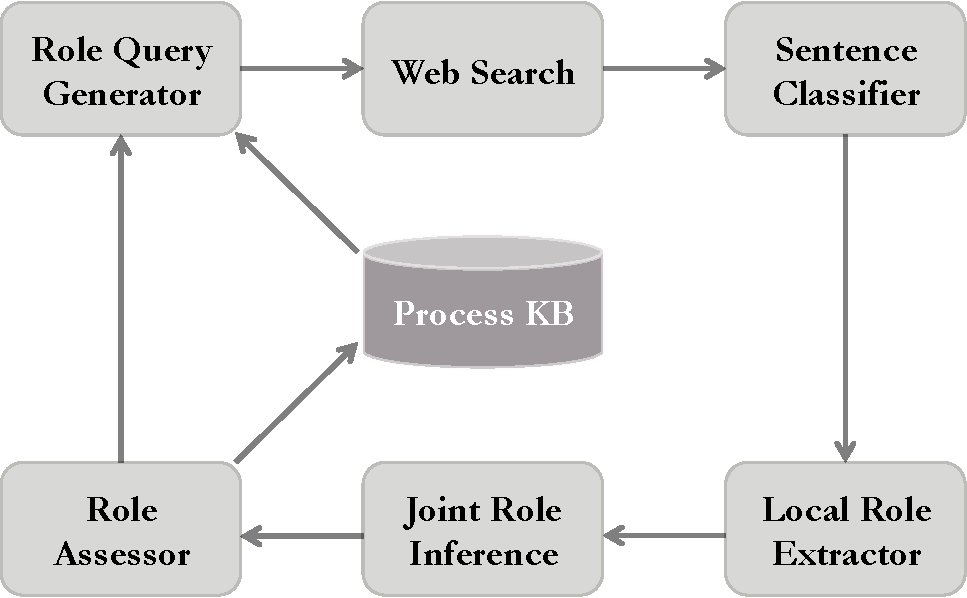
\includegraphics[width=2.49in,height=2.45in]{figures/architecture} 	
	\caption{\label{fig:architecture} {Process KB Acquisition: Proposed Architecture}}
	\end{center}
\end{figure}

\section{ProcIteRoles: Architecture}

\sys\ allows for targeted iterative acquisition and refinement of process roles.
The central idea is to collect high quality sentences and roles and iteratively expand the acquisition to include
additional sentences and other roles. 

Figure~\ref{fig:architecture} shows the architecture of the acquisition process. 
Using simple query patterns we search for sentences that express roles with highly regular lexical cues. 
A sentence filter addresses sense issues and to remove malformed sentences.
The filtered sentences are then processed through a pattern-based extractor that identifies and scores the candidate roles. 
In parallel, the sentences are also aligned to identify lexical units that should play similar semantic roles in the sentences. 
A joint inference module then provides a collective label assignment for all the sentences. 
The extracted roles are then assessed in conjunction with the existing roles. 
The assessor determines which roles should be added to the KB and also determines which roles need further additions. 
New query patterns are created for the roles that need addition and whole procedure is repeated again. 

In the subsequent sections, we describe each component in greater detail.

\section{Sentence Gathering}

\sys\ will leverage the vastness of the web to build a targeted collection of sentences that expresses roles of interest.
There are two key challenges to address in gathering relevant sentences:
\begin{itemize}
\item {\bf Relevance} -- We want to find sentences that describe the target process of interest. 
The vastness of the web also means that there is information on nearly any possible interpretation of the words used to describe the process. 
For instance if we are interested in the process {\em crop fertilization}, we might also find information on {\em fertilization} in the reproductive sense, 
or in other metaphorical uses such as {\em cross fertilization of ideas}. 
Also, the target sense may not be a dominant sense on the web. 
Constructing effective keyword queries is therefore critical for finding relevant information.
\item {\bf Role Coverage} -- We want to find sentences that cover all applicable roles that convey the desired information via simple expected constructions.
Some roles are often expressed via highly regular lexico-syntactic constructions. 
On the other hand, roles such as {\em x} can be expressed in many different ways. 
Again with the vastness of the web, constructing effective role patterns is critical for finding useful sentences. 
\end{itemize}

To address these challenges we propose two strategies. First, we target definitional sentences which convey the most salient information. Second, we espouse a feedback strategy that leverages high quality sentences gathered in the earlier phases to guide search in the later stages.

\subsection{Querying}

We propose to investigate simple but effective query pattern formulation methods. 
On a related task, our prior work had explored techniques that can find sentences that convey information about different aspects with respect to a topic (e.g., biographical aspects of a person). 
Our preliminary work shows that simple lexical templates e.g., "<process name> is the process by which" can yield high quality {\em definitional} sentences about processes. 
We use additional lexical templates for roles with regular lexicon-syntactic constructions e.g., "<process name> causes" is an effective pattern to find sentences that express the {\em result} roles of processes. The key challenge is to figure out querying patterns for roles with diverse lexical realizations. We propose adopting the standard bootstrapping approach used in relation extraction techniques to borrow functional patterns that introduce roles in other processes. Bootstrapping is known to introduce noise and topic drift issues. However, our approach doesn't entirely rely on the patterns alone. Rather we propose strong scoring and filtering mechanisms that can remove noise introduced via bootstrapping.

\subsection{Scoring and Filtering}

To account for the challenges in relevance, we seek to build a distributional context model that is seeded with some domain corpus. This model is then refined iteratively to allow for role coverage. 
Sentences from the web have high variance in quality and relevance. 

\section{Role Extraction}

Many different approaches have been investigated for role labeling.
The learning formulations studied range from pipelined classification approaches~\cite{gildea2002automatic,bjorkelund2009multilingual}, 
efficient structured and joint inference~\cite{koomen2005generalized,tackstrom2015efficient}, to end-to-end deep learning architectures~\cite{foland2015dependency}.
Many different lexico-syntactic features, such as dependency paths and n-gram contexts, provide weak evidences for determining semantic roles~\cite{gildea2002automatic}. 
Because these path-based and n-gram features are sparse, these supervised techniques require large amounts of training data. 
Semi-supervised and unsupervised approaches have been proposed as a means to address the training data problem~\cite{furstenau-emnlp2009,klementievsemi}.

The focus of these approaches have been to build a SRL system that can identify the roles mentioned in a sentence. 
Our requirement is subtly different. We need to build a mechanism for acquiring the typical role fillers for a given process. 
First, we formulate a simpler local classification task that avoids the need for learning over role and predicate specific patterns. 
Starting with sentences that are likely to contain a specific role and a candidate text span from the sentence, 
we pose a classification task to determine if the candidate  is indeed expressing role of interest. 
Then, we pose a joint inference task over multiple sentences, which allows us to use role decisions on similar 
text spans to influence each other. 

\subsection{Local Role Extraction}

We set up a local (within sentence per role) extraction task. Relying on the patterns alone is problematic. Hand authored patterns, especially specifying the expected syntactic structure of the argument is quite limiting. Instead we generate many possible arguments that match a range of weakly indicative argument patterns and train a classifier. 

The inputs are a sentence $S$, the role $R$ for which it was retrieved, and the role pattern $X_R$ that it matches, and a set of candidate spans $C$.
The task is to predict if for each span if it is expressing the role of interest. 

We adopt the standard SRL features such as clause, dependency path features, and n-gram context features~\cite{gildea2002automatic,koomen2005generalized}. 
We explore two types of extensions that are specific to our setting:
\begin{itemize}

\item Different from a standard SRL setting, we seek identification of roles with respect to a canonical realization of the process. 
One can view this task as finding a mapping from predicate-specific semantic role to the process-specific role. 
To this end, we use an SRL system trained on PropBank data to identify predicate level semantic roles and use those as features to derive this mapping.
Similarly, the frames that are evoked by the predicates in the sentence also provide important signals. For example, knowing that there is a conversion 
frame in a sentence increases the possibility of finding a result of a change of state of process like evaporation. 

\item Also we have strong expectations on {\em how} the argument is realized because the sentence is retrieved via a specific query pattern.
This allows us to encode features that test if the expectations are met. [{\bf Explain w/ an example}]

\end{itemize}


%Rather than focus on joint role inference at a sentence level, we explore joint inference across sentences.
%This task is different from the standard SRL setting in two ways. 
%First, we have a strong expectation on {\em how} the argument is realized because the sentence is retrieved via a specific query pattern.
%This allows us to encode features that test if the expectations are met. 
%Second, the task of identifying roles is not specific to a particular predicate. 
%Rather, the roles are identified with respect to a canonical realization of the process. 
%One can view this task as that of mapping from the predicate-specific semantic role to the process-specific role. 

\subsection{Joint Role Inference}

Within sentence joint role inference has been shown to help SRL~\cite{punyakanok2004srl,koomen2005generalized}.
Since our objective is to extract knowledge from multiple sentences, we propose to also exploit joint inference of roles across sentences. Local role extraction allows to reliably identify whether the specified role is expressed by the candidate text spans. However, this local classification is often inadequate because some cue patterns are ambiguous. For example, "evaporates into <x>" can match "steam" which is a {\em result} or "atmosphere" which is a {\em location}. Relying on the extraction pattern alone is problematic. Therefore, we propose to leverage role predictions on other similar text spans to improve inference. 


{\bf Formalism}

The key premise is that aligned text spans in similar sentences should be assigned same roles. This idea had been successfully used in semi-supervised and unsupervised settings to increase training data for SRL~\cite{furstenau-emnlp2009,furstenau2012semi,lang-emnlp2011}. We adopt it for joint inference over test sentences, similar to the transductive learning approaches~\cite{?}.

We extend an ILP-based formalism which has been shown to successfully model within sentence joint inference for SRL~\cite{punyakanok2004srl}. We add 1) a penalty term to the maximization objective that penalizes assignments that violate smoothness of labeling, 2) constraints that effectively fix labels from the local extractor for certain roles. 

As noted earlier, the local extractor scores each text span $t_{i,k}$ from sentence $S_k$ on how likely it is to belong to the role $r_j$. We use indicator variables to denote role assignment. $z_{ijk}$ represents if the text span $t_{ik}$ in sentence $S_k$ is assigned the role $r_j$. Formally, the inference aims to find the best joint assignment to set of indicator variables $\mathbb{z}$ that maximizes the following objective function:

\begin{align*}
%\sum_{t_{ik}} \sum_{r_j} 
 \arg\max_{\mathbf{z}}  \sum_{i,j,k} z_{ijk} \cdot \rho(t_{ik}, r_j) \cdot \lambda_{j}
	&- \beta \left\{ \sum_{i,k,l,m} \sigma(t_{ik}, t_{lm}) \left(\sum_{c \in |R|} |z_{ick} - z_{lcm}| \right) \right\}\\
\mbox{subject to} \\
\forall z_{ick} \in \mathbf{z}, \sum_{c = 1}^{|R|} z_{ick} \le 1  &\mbox{[A span gets only one role.]}\\
\forall S_k \forall c \in |R|, \sum_{t_{ik} \in S_k} z_{ick} \le 1  & \mbox{[Roles are not repeated.]} \\
 \cdots&  \mbox{[Other within sentence constraints.]}
\end{align*}

{\bf Sentence and Text Span Alignment}

The effectiveness of the joint inference relies on the ability to identify text spans in different sentences that should get the same role. 
Prior work explored a dependency graph-based approach to align predicate-argument structures in sentences. A linear combination of the overlap in lexical and syntactic structures of the candidate text spans is used to evaluate whether they should get the same roles~\cite{furstenau-emnlp2009,furstenau2012semi,lang-naacl2010}.
This scoring function is used to transfer roles from a labeled sentence to an unlabeled sentence (semi-supervised setting) or to induce roles as clusters of arguments (unsupervised setting). 

A key difference in our setting is that there are different sub-groups of sentences with different alignment characteristics. 
{\em Definition} sentences describe the process in terms of classes of entities and {\em instance} sentences which involve specific entities.
Aligning definitional sentences is quite different from aligning definitions with instances or instances with other instances. 
Instances involve completely different entities which may not align via direct entailment but may align as substitutable siblings.
Also, instances often tend to involve other non-essential information with respect to the process, 
whereas definitions are compact and tend to contain the most salient bits of information. 
To account for these differences we consider two extensions. Use different sets of weights and different similarity functions to combine the scores based on the types of sentences being aligned.

\begin{align*}
\sigma(t_{ik}, t_{lm}, u, v)	= \alpha_{uv} \cdot lexsim_{uv}(t_{ik}, t_{lm}) + (1 - \alpha_{uv}) \cdot synsim_{uv}(t_{ik}, t_{lm})\\
\end{align*}

[{\bf Consider changing this to a trained classifier. Use sentence patterns rather than definition or instance sentence distinction.}]

\section{Role Aggregation and Assessment}

Inference yields a set of roles that can be reliably identified from the input set of sentences. 
The knowledge thus gathered is limited by the query patterns that we used to retrieve the sentences in the first place. To expand the knowledge further, we propose an iterative procedure that learns from the inferred roles. 

\subsection{Aggregation}
First, given the current state of the knowledge base and newly inferred roles we devise a simple aggregation procedure that consolidates the roles -- resolving any inconsistencies between the different iterations\footnote{
It is possible to infer new roles with respect to the KB at each iteration, it can introduce many variables 
in inference and render it inefficient.
}.

\subsection{Assessment}

We inspect the KB to identify roles that apply for a specific process based on the confidences of the inferred roles. 
Note that we do not make any assumptions a priori about what roles apply to a process. 
Further not all roles maybe covered by the roles vocabulary. For example, ....
We identify regular syntactic signatures that are not classified into existing roles and use them to derive new knowledge.


need to be filled, and pass them on to the sentence gathering components for expansion.


%instantiate new patterns to identify better sentences. The idea is to evaluate lexical alternatives that can form better queries to identify sentences. For example, sentences describing instances of conduction of heat are better found by adding {\em heat}. This type of query expansion using pseudo-relevance feedback is a well studied technique in information retrieval. We consider a restricted version of this problem, where are looking to instantiate existing query templates. 





% !TEX root =  main.tex
\section{Role Assessment and Discovery}

Inference yields a set of role fillers that can be reliably identified from the input set of sentences. 
The yield is limited by the set of roles and the query patterns used to retrieve sentences for these roles.

{\bf Assessment}

To expand the knowledge further, we propose an iterative procedure that learns from the inferred roles to find new query patterns. 
Traditional bootstrapping methods coupled with query expansion techniques from information retrieval 
can be exploited to instantiate query templates with new patterns derived from the retrieved sentences. 
The new query patterns are then used to repeat the entire procedure to derive new fillers. 

The iterative procedure however can yield role fillers that are inconsistent with roles obtained from previous iterations.
While it is possible to infer new roles jointly with the current KB at each iteration, it can introduce too many variables in inference and render it inefficient.
Therefore, we propose a simple aggregation procedure that consolidates the roles by effectively resolving any inconsistencies between the different iterations.
%Last we will also explore methods that automatically assesses the generated knowledge in terms of coverage and quality

{\bf Role Discovery and Refinement}

At each iteration we will also inspect if there are any new roles that need to be added to the role set.
For many processes there are specific important roles that do not fit any of the general roles. Some examples:
	\begin{itemize}
		\item {\em Phototropism} is the mechanism by which plants grow towards a light source. 
		The notion of a target {\em light source} and the {\em direction} or {\em orientation} of the growth
		are critical for distinguishing positive and negative phototropism. However, neither notion fits
		with any of the existing roles. 
	\item {\em Heat transfer} processes such as radiation have notion of a {\em medium}, 
		which is critical for distinguishing between instances such as convection and radiation
		Again medium doesn't fit with any existing roles. 
	\end{itemize}

Our objective is similar to the goals of prior work on unsupervised role induction. They use a deterministic procedure for candidate argument identification and clustered syntactic signatures of these arguments to induce roles. However, unlike the standard unsupervised setting, we have a set of roles that have been identified already. Further, we find that most of these process specific new roles tend to be realized via prepositional, noun-noun, or other noun modifier relations that attach to one of the existing roles. Information about how these candidates are related to currently identified roles is likely to help.

\begin{itemize}
\item We propose to investigate methods for breaking coarse-grained roles into multiple sub-roles.
 and preposition relation extraction tools 

We use two sources for identifying candidates. 
First, we obtain candidates from the local extraction pipeline that were assigned low scores by the inference and then we extend it with candidates from a separate PropBank style argument identification pipeline~\cite{}. Second, we also inspect role fillers for existing roles that can be broken up into fine-grained roles. For example, "towards a light source" can be further split into two roles one relating to the "direction" of the growth and the other relating to the goal "light source".

\item Having identified candidates we iterate through the pipeline to find additional sentences that contain these candidates and the core roles or predicates for the process. Following prior role induction work, we extract a context signature for each candidate and cluster the candidates that are realized with similar contexts. As mentioned earlier, we propose to also use the semantic role context of the candidates. 

\end{itemize}








% !TEX root =  main.tex
\section{Evaluation}

Our primary motivation is to compose knowledge that is necessary for grade-level science questions.
Therefore we propose both an intrinsic evaluation that measures the accuracy of the extracted roles, and an external evaluation where we assess the utility of the roles in question answering.

\subsection{KB Evaluation}

Our goal is to acquire knowledge about processes along relevant role dimensions.
[{\bf To be filled...]}


\subsection{Question Answering using Semantic Roles}

{\bf Testbed}
Following Clark et al., 2014, we propose to build a large collection of multiple-choice questions at different grade levels. 
In prior work we leveraged existing collections to select questions. 
To effectively test the utility of our approach, we propose to create two types of questions in increasing levels of difficultly: 1) Questions that test ability to recognize instances of processes. 2) Questions that require ability to reason about the instance. We will limit the reasoning questions to those that are effectively achieved by following simple axioms defined over the semantic roles. [Example???]

Creating these questions is a difficult task for non-experts. We propose to work with the graduate students in the Department of Education at Stony Brook to collect questions and question templates. 
Once we have generate question templates that specify what kind of understanding is to be tested, we can scale out the question acquisition process via crowd sourcing. 

{\bf Method}

We use a simple approach to evaluate the utility of semantic roles for question answering. 
For the recognition questions we will follow our prior work, where we build a supervised role labeler 
and use it to parse the question to extract a role based representation. 
Then for each answer option we match the extracted roles against the roles available in the database. 

For reasoning questions, we will utilize the above approach to first recognize the process and identify the roles mentioned in the question. We will utilize hand-written axioms defined over the roles. [Example.?]



% !TEX root =  main.tex
\section{Development Plan and Timeline}

The project will proceed in four stages. 1) Representation design 2) Extraction methods 3) Expansion methods 4) Curation and release. The developed components will be evaluated and improved continually. The research plan in calendar years is shown below:\\
{\bf Year 1: }
\begin{enumerate}[noitemsep,nolistsep]
\item Inferential needs gathering and representation design.
\item Implement sentence gathering. 
\item Extraction and joint inference methods.
\item Intrinsic evaluation of the knowledge base.
\end{enumerate}
{\bf Year 2:}
\begin{enumerate}[noitemsep,nolistsep]
\item Investigate methods for improving joint inference and iterative expansion.
\item Expansion of the KB to all target concepts and evaluation of the resulting knowledge base and 
\item Curation and release of knowledge base. Open source release of the software and web service.
\end{enumerate}
\vspace{-1em}

\section{Broader Impacts of the Proposed Activities}

Knowledge about processes is fundamental to our understanding of the world and vital for AI systems that interact with the world and with humans.  Computational representations of scientific knowledge has tremendous applications in improving access to critical information, as well as in accelerating discovery and research processes. Moreover AI systems are increasingly adopted for use in many types of decision making in critical areas such as technology, science, and medicine. Knowledge based reasoning is crucial for building systems that have the ability to explain their decisions or predictions. Such systems require an understanding how to represent knowledge in a form that lends itself to computational reasoning for complex tasks.

\subsection{Curriculum Development Activities}

The PI teaches grad-level Introduction to Natural Language Processing, and Advanced Topics in Computational Linguistics. 
With advent of big data ecosystem understanding and extracting knowledge is becoming increasingly relevant in industry.
I plan to teach a course centered around the core concepts of knowledge representation, and scalable extraction techniques for knowledge. This course is relevant for both Masters and PhD students. Most NLP-based technology companies and technology companies with a large web presence have a need for extracting and organizing knowledge from their user engagement data. This course will provide a basic overview of a distributed information extraction pipeline, persistence, and building applications that rely on the extracted data. 

\subsection{Community Outreach}

There is an increased enthusiasm for advanced placement computer science courses in the high schools in local communities. 
The proposed project deals with computational representations of scientific processes discussed in grade level sciences. 
This provides an unique opportunity to introduce computer science concepts using an application domain that they are familiar with.
The familiarity and the far reaching impact possibilities provide an excellent platform to attract the attention of high school students.
The PI plans to offer introductory technical lectures, and project opportunities to engage high school students in the context of the proposed project. 

\section{Prior NSF Support}

Dr. Niranjan Balasubramanian has broad expertise in information extraction, esp. in large scale knowledge generation and its application to complex NLP tasks but has not received prior support from NSF. 

\newpage
{\small
\bibliographystyle{plain}
\bibliography{main}
}
\end{document}
